\documentclass{standalone}
\usepackage{tikz}
\usetikzlibrary{patterns, positioning}

\begin{document}
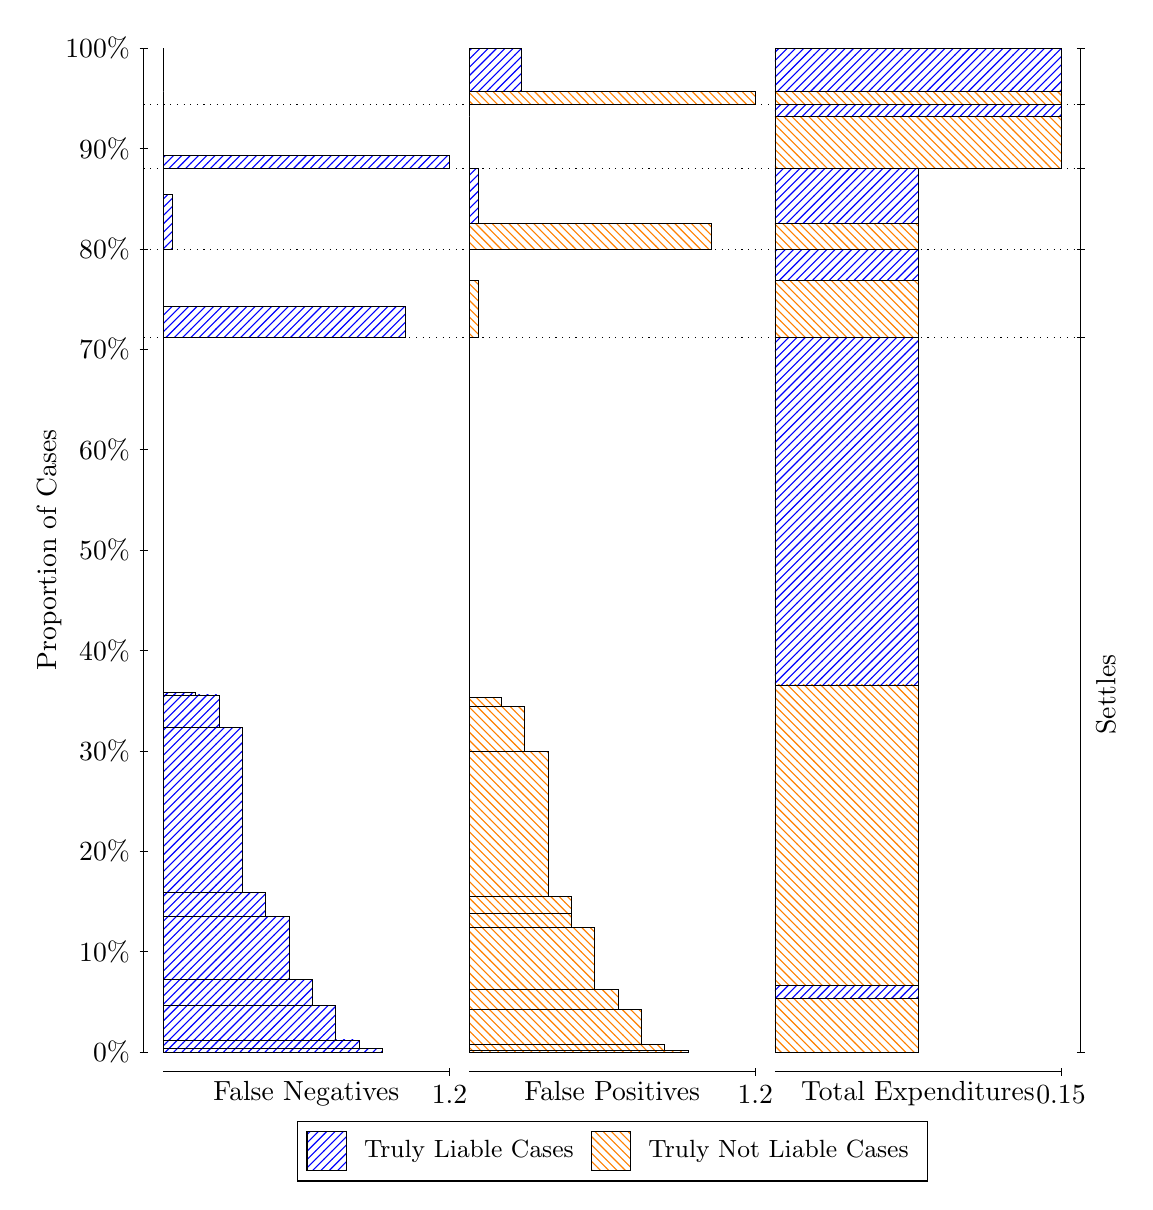
\begin{tikzpicture}
\draw[black, very thin] (1.5,1.75) -- (1.5,14.5);
\node[rotate=90, anchor=center] at (0.3, 8.125) {Proportion of Cases};
\draw[black, very thin] (1.45,1.75) -- (1.55,1.75);
\node[anchor=east] at (1.45, 1.75) {0\%};
\draw[black, very thin] (1.45,3.025) -- (1.55,3.025);
\node[anchor=east] at (1.45, 3.025) {10\%};
\draw[black, very thin] (1.45,4.3) -- (1.55,4.3);
\node[anchor=east] at (1.45, 4.3) {20\%};
\draw[black, very thin] (1.45,5.575) -- (1.55,5.575);
\node[anchor=east] at (1.45, 5.575) {30\%};
\draw[black, very thin] (1.45,6.85) -- (1.55,6.85);
\node[anchor=east] at (1.45, 6.85) {40\%};
\draw[black, very thin] (1.45,8.125) -- (1.55,8.125);
\node[anchor=east] at (1.45, 8.125) {50\%};
\draw[black, very thin] (1.45,9.4) -- (1.55,9.4);
\node[anchor=east] at (1.45, 9.4) {60\%};
\draw[black, very thin] (1.45,10.675) -- (1.55,10.675);
\node[anchor=east] at (1.45, 10.675) {70\%};
\draw[black, very thin] (1.45,11.95) -- (1.55,11.95);
\node[anchor=east] at (1.45, 11.95) {80\%};
\draw[black, very thin] (1.45,13.225) -- (1.55,13.225);
\node[anchor=east] at (1.45, 13.225) {90\%};
\draw[black, very thin] (1.45,14.5) -- (1.55,14.5);
\node[anchor=east] at (1.45, 14.5) {100\%};

\draw[black, very thin] (13.4,1.75) -- (13.4,14.5);
\draw[black, very thin] (13.35,1.75) -- (13.45,1.75);
\node[anchor=west] at (13.35, 1.75) {};
\draw[black, very thin] (13.35,10.828) -- (13.45,10.828);
\node[anchor=west] at (13.35, 10.828) {};
\draw[black, very thin] (13.35,11.944) -- (13.45,11.944);
\node[anchor=west] at (13.35, 11.944) {};
\draw[black, very thin] (13.35,12.974) -- (13.45,12.974);
\node[anchor=west] at (13.35, 12.974) {};
\draw[black, very thin] (13.35,13.788) -- (13.45,13.788);
\node[anchor=west] at (13.35, 13.788) {};
\draw[black, very thin] (13.35,14.5) -- (13.45,14.5);
\node[anchor=west] at (13.35, 14.5) {};

\draw[black, very thin, pattern color=blue, pattern=north east lines] (1.75,1.75) rectangle (4.5306,1.7913);
\draw[black, very thin, pattern color=blue, pattern=north east lines] (1.75,1.7913) rectangle (4.234,1.9046);
\draw[black, very thin, pattern color=blue, pattern=north east lines] (1.75,1.9046) rectangle (3.9374,2.3371);
\draw[black, very thin, pattern color=blue, pattern=north east lines] (1.75,2.3371) rectangle (3.6408,2.6697);
\draw[black, very thin, pattern color=blue, pattern=north east lines] (1.75,2.6697) rectangle (3.3442,3.4757);
\draw[black, very thin, pattern color=blue, pattern=north east lines] (1.75,3.4757) rectangle (3.0476,3.7797);
\draw[black, very thin, pattern color=blue, pattern=north east lines] (1.75,3.7797) rectangle (2.751,5.8722);
\draw[black, very thin, pattern color=blue, pattern=north east lines] (1.75,5.8722) rectangle (2.4544,6.285);
\draw[black, very thin, pattern color=blue, pattern=north east lines] (1.75,6.285) rectangle (2.1578,6.3201);
\draw[black, very thin, pattern color=orange, pattern=north west lines] (1.75,6.3201) rectangle (1.75,10.828);
\draw[black, very thin, pattern color=blue, pattern=north east lines] (1.75,10.828) rectangle (4.8272,11.221);
\draw[black, very thin, pattern color=orange, pattern=north west lines] (1.75,11.221) rectangle (1.75,11.944);
\draw[black, very thin, pattern color=blue, pattern=north east lines] (1.75,11.944) rectangle (1.8612,12.644);
\draw[black, very thin, pattern color=orange, pattern=north west lines] (1.75,12.644) rectangle (1.75,12.974);
\draw[black, very thin, pattern color=blue, pattern=north east lines] (1.75,12.974) rectangle (5.3833,13.132);
\draw[black, very thin, pattern color=orange, pattern=north west lines] (1.75,13.132) rectangle (1.75,13.788);
\draw[black, very thin, pattern color=orange, pattern=north west lines] (1.75,13.788) rectangle (1.75,13.945);
\draw[black, very thin, pattern color=blue, pattern=north east lines] (1.75,13.945) rectangle (1.75,14.5);
\draw[black, very thin, pattern color=orange, pattern=north west lines] (5.6333,1.75) rectangle (8.4139,1.7697);
\draw[black, very thin, pattern color=orange, pattern=north west lines] (5.6333,1.7697) rectangle (8.1173,1.8495);
\draw[black, very thin, pattern color=orange, pattern=north west lines] (5.6333,1.8495) rectangle (7.8207,2.2885);
\draw[black, very thin, pattern color=orange, pattern=north west lines] (5.6333,2.2885) rectangle (7.5241,2.5434);
\draw[black, very thin, pattern color=orange, pattern=north west lines] (5.6333,2.5434) rectangle (7.2276,3.3313);
\draw[black, very thin, pattern color=orange, pattern=north west lines] (5.6333,3.3313) rectangle (6.931,3.5085);
\draw[black, very thin, pattern color=orange, pattern=north west lines] (5.6333,3.5085) rectangle (6.931,3.7247);
\draw[black, very thin, pattern color=orange, pattern=north west lines] (5.6333,3.7247) rectangle (6.6344,5.5711);
\draw[black, very thin, pattern color=orange, pattern=north west lines] (5.6333,5.5711) rectangle (6.3378,6.1431);
\draw[black, very thin, pattern color=orange, pattern=north west lines] (5.6333,6.1431) rectangle (6.0412,6.2581);
\draw[black, very thin, pattern color=blue, pattern=north east lines] (5.6333,6.2581) rectangle (5.6333,10.828);
\draw[black, very thin, pattern color=orange, pattern=north west lines] (5.6333,10.828) rectangle (5.7446,11.551);
\draw[black, very thin, pattern color=blue, pattern=north east lines] (5.6333,11.551) rectangle (5.6333,11.944);
\draw[black, very thin, pattern color=orange, pattern=north west lines] (5.6333,11.944) rectangle (8.7105,12.275);
\draw[black, very thin, pattern color=blue, pattern=north east lines] (5.6333,12.275) rectangle (5.7446,12.974);
\draw[black, very thin, pattern color=orange, pattern=north west lines] (5.6333,12.974) rectangle (5.6333,13.631);
\draw[black, very thin, pattern color=blue, pattern=north east lines] (5.6333,13.631) rectangle (5.6333,13.788);
\draw[black, very thin, pattern color=orange, pattern=north west lines] (5.6333,13.788) rectangle (9.2667,13.945);
\draw[black, very thin, pattern color=blue, pattern=north east lines] (5.6333,13.945) rectangle (6.3007,14.5);
\draw[black, very thin, pattern color=orange, pattern=north west lines] (9.5167,1.75) rectangle (11.333,2.437);
\draw[black, very thin, pattern color=blue, pattern=north east lines] (9.5167,2.437) rectangle (11.333,2.5916);
\draw[black, very thin, pattern color=orange, pattern=north west lines] (9.5167,2.5916) rectangle (11.333,6.4128);
\draw[black, very thin, pattern color=blue, pattern=north east lines] (9.5167,6.4128) rectangle (11.333,10.828);
\draw[black, very thin, pattern color=orange, pattern=north west lines] (9.5167,10.828) rectangle (11.333,11.551);
\draw[black, very thin, pattern color=blue, pattern=north east lines] (9.5167,11.551) rectangle (11.333,11.944);
\draw[black, very thin, pattern color=orange, pattern=north west lines] (9.5167,11.944) rectangle (11.333,12.275);
\draw[black, very thin, pattern color=blue, pattern=north east lines] (9.5167,12.275) rectangle (11.333,12.974);
\draw[black, very thin, pattern color=orange, pattern=north west lines] (9.5167,12.974) rectangle (13.15,13.631);
\draw[black, very thin, pattern color=blue, pattern=north east lines] (9.5167,13.631) rectangle (13.15,13.788);
\draw[black, very thin, pattern color=orange, pattern=north west lines] (9.5167,13.788) rectangle (13.15,13.945);
\draw[black, very thin, pattern color=blue, pattern=north east lines] (9.5167,13.945) rectangle (13.15,14.5);
\draw[black, dotted] (1.5,10.828) -- (13.4,10.828);
\draw[black, dotted] (1.5,11.944) -- (13.4,11.944);
\draw[black, dotted] (1.5,12.974) -- (13.4,12.974);
\draw[black, dotted] (1.5,13.788) -- (13.4,13.788);
\draw[black, very thin] (1.75,1.5) -- (5.3833,1.5);
\node[anchor=north] at (3.5667, 1.5) {False Negatives};
\draw[black, very thin] (5.3833,1.45) -- (5.3833,1.55);
\node[anchor=north] at (5.3833, 1.45) {1.2};

\draw[black, very thin] (5.6333,1.5) -- (9.2667,1.5);
\node[anchor=north] at (7.45, 1.5) {False Positives};
\draw[black, very thin] (9.2667,1.45) -- (9.2667,1.55);
\node[anchor=north] at (9.2667, 1.45) {1.2};

\draw[black, very thin] (9.5167,1.5) -- (13.15,1.5);
\node[anchor=north] at (11.333, 1.5) {Total Expenditures};
\draw[black, very thin] (13.15,1.45) -- (13.15,1.55);
\node[anchor=north] at (13.15, 1.45) {0.15};

\node[black, centered, rotate=90] at (13.72, 6.2891) {Settles};





\draw (7.449999999999999,1.5) node[draw=none] (baseCoordinate) {};
\begin{scope}[align=center]
        \matrix[scale=0.5, draw=black, below=0.5cm of baseCoordinate, nodes={draw}, column sep=0.1cm]{
            \node[rectangle, draw, minimum width=0.5cm, minimum height=0.5cm, pattern=north east lines, pattern color=blue] {}; &
            \node[draw=none, font=\small] (B) {Truly Liable Cases}; &
            \node[rectangle, draw, minimum width=0.5cm, minimum height=0.5cm, pattern=north west lines, pattern color=orange] {}; &
            \node[draw=none, font=\small] (B) {Truly Not Liable Cases}; \\
            };
\end{scope}

\end{tikzpicture}
\end{document}